\documentclass[aps,pre,12pt,preprint,onecolumn,showpacs,showkeys]{revtex4-1}

% Setting up Chinese handling.
\usepackage{fontspec,xeCJK}

% Setting up fonts.
% PLEASE MODIFY ALL THESE FONT NAMES ACCORDING TO YOUR FONT
% INSTALLATION AND PERFERENCE.

% Setting up main fonts and mono fonts.
\setmainfont{Liberation Serif}
\setmonofont{Liberation Mono}
% SimSun is required font for the main body of the text.
\setCJKmainfont[AutoFakeBold=5,AutoFakeSlant]{SimSun}
\setCJKmonofont[AutoFakeBold=2,AutoFakeSlant]{SimHei}

% Setting up alternative font families.
% Note that these three fonts below are required fonts in document
% title, section headings and figure captions.
\newCJKfontfamily\heiti[AutoFakeBold=2,AutoFakeSlant]{SimHei}
\newCJKfontfamily\fangsong[AutoFakeBold=5,AutoFakeSlant]{FangSong}
\newCJKfontfamily\kaiti[AutoFakeBold=5,AutoFakeSlant]{KaiTi}

% Setting up paragraph indent.
\parindent 2em

% Setting up macros for Chinese-style font size setting.
\newcommand{\fseight}{\fontsize{5.02}{6.02}\selectfont}
\newcommand{\fsseven}{\fontsize{5.52}{6.62}\selectfont}
\newcommand{\fsssix}{\fontsize{6.52}{7.83}\selectfont}
\newcommand{\fssix}{\fontsize{7.53}{9.03}\selectfont}
\newcommand{\fssfive}{\fontsize{9.03}{10.84}\selectfont}
\newcommand{\fsfive}{\fontsize{10.54}{12.65}\selectfont}
\newcommand{\fssfour}{\fontsize{12.05}{14.45}\selectfont}
\newcommand{\fsfour}{\fontsize{14.05}{16.86}\selectfont}
\newcommand{\fssthree}{\fontsize{15.06}{18.07}\selectfont}
\newcommand{\fsthree}{\fontsize{16.06}{19.27}\selectfont}
\newcommand{\fsstwo}{\fontsize{18.07}{21.68}\selectfont}
\newcommand{\fstwo}{\fontsize{22.08}{26.50}\selectfont}
\newcommand{\fssone}{\fontsize{24.09}{28.91}\selectfont}
\newcommand{\fsone}{\fontsize{26.10}{31.32}\selectfont}
\newcommand{\fsszero}{\fontsize{36.14}{43.36}\selectfont}
\newcommand{\fszero}{\fontsize{42.16}{50.59}\selectfont}

% Replace words to Chinese corespondence.
\renewcommand\appendixname{附录}
\renewcommand\abstractname{}
\renewcommand\tablename{表}
\renewcommand\figurename{图}

% Replace words in revtex4-1 to Chinese corespondence.
\makeatletter
\def\@pacs@name{\heiti\fssfour \textbf{PACS码:}\normalfont}
\def\@keys@name{\heiti\fssfour \textbf{关键词:}\normalfont}
\def\Dated@name{日期:}
\def\Received@name{\fssfive 接收 }
\def\Revised@name{\fssfive 修订 }
\def\Accepted@name{\fssfive 采纳 }
\def\Published@name{\fssfive 发表 }
\makeatother

% Change label style of enumerate.
\renewcommand{\labelenumi}{\alph{enumi}.}

% Setting up geometry.
\usepackage{geometry}
\geometry{top=2.54cm,bottom=2.54cm,left=3cm,right=3cm}

% Setting up line space.
\usepackage{setspace}
\linespread{1.6}

% Setting up hyperreferences.
\usepackage{hyperref}
\hypersetup{colorlinks=true}

% Setting up styles for section headings.
\usepackage{titlesec}
\titleformat*{\section}{\bf\fangsong\fsfour}
\titleformat*{\subsection}{\bf\fangsong}

% Loading packages for image handling.
\usepackage{subfig}
\usepackage{graphicx,psfrag,epsfig}

% Setting up caption styles.
\usepackage{caption}
\DeclareCaptionFont{kaiti}{\kaiti}
\DeclareCaptionFont{bfheiti}{\bf\heiti}
\captionsetup{font=small,format=plain,labelfont=bfheiti,%
  textfont=kaiti,justification=raggedright,%
  singlelinecheck=false}

% Loading packages for math typings.
\usepackage{amsmath,amsfonts,amssymb,amsthm,bm,upgreek}
\usepackage[mathscr]{eucal}


\begin{document}

% Title and author info.
\title{\bf\heiti\fsthree 用快速电子验证动量-动能的相对论关系预习报告\vspace{15mm}}
\author{\fangsong\fsfour 智朝晖\vspace{2mm}}
\affiliation{\normalfont\fssfour 北京航空航天大学物理学院2020级本科生~~~~~~学号:
  {20377365}\vspace{2mm}}
\date{2022年9月12日}
\keywords{动量-动能关系,$\beta$衰变,$\beta$粒子,狭义相对论}
\email{20377365@buaa.edu.cn; {17741852357}}

% Abstract.
\begin{abstract}
  \vspace{10mm}
  \begin{spacing}{1.5}
    \fssfour
    经典力学和电磁学以及光学之间的矛盾,促成了狭义相对论理论的诞生.狭义
    相对论理论对于高速物体的运动,和经典力学对于物体的动量-动能关系,给
    出了不同的预计.本实验通过测量高能$\beta$粒子的动量和动能,验证了狭
    义相对论对于高速运动物体动量-动能关系的预计.并且通过对于空气中
    $\beta$粒子运动的研究,证明了$\beta$粒子在空气中运动时会损失能量.
  \end{spacing}
\end{abstract}

% The main body of the document goes from here.
\maketitle
\fssfour

% Instructions on writing.


\section{实~~验~~原~~理}

狭义相对论的理论框架基于如下两个假设建立:

\begin{enumerate}
\item 爱因斯坦相对性原理: 所有物理规律在所有惯性参考系中具有完全相同的
  形式.
\item 光速不变原理: 在所有惯性参考系中光在真空的速度恒定为$c$,它与光源
  和参考系的运动无关.
\end{enumerate}

基于这两个假设,可以推导出洛伦兹变换.洛伦兹变换作为一种变换关系,用于联系
不同惯性参考系之中的运动量.同时,如若引入$x_1 = x, x_2 = y, x_3 = z,
x_4 = ict$,根据洛伦兹变换,可以发现在变换中存在一个不变量$x_1^2 + x_2^2
+ x_3^2 + x_4^2$,从而洛伦兹变换可以看成复四维时空$(x_1, x_2, x_3,
x_4)$之中的转动.

另一方面,根据相对性原理,任何物理规律在不同的惯性系中都具有相同的形式,
因此表达物理规律的方程必须满足在洛伦兹变换形式下不变,称为洛伦兹变换的
协变性.由于洛伦兹变换可以看成上述复四维时空中的转动,因此,若能将物理量
和物理规律的表达式以该四维时空中的形式进行表述,可以使得表述本身更加清
晰、简明.

首先,四维时空中的坐标平方和以及微位移平方都是洛伦兹不变量,即
\begin{equation}
  \label{eq:const1}
  x_1^2 + x_2^2 + x_3^2 + x_4^2 = \text{const.}
\end{equation}
以及
\begin{equation}
  \label{eq:const2}
  (dx_1)^2 + (dx_1)^2 + (dx_1)^2 + (dx_1)^2 = \text{const.}
\end{equation}
从这个角度上来看,由于洛伦兹变换是四维时空中的转动,因此可以定义四维
位矢和四维微位移,即
\begin{equation}
  \label{eq:4vecr}
  \bm{R} = (x,y,z,ict)
\end{equation}
以及
\begin{equation}
  \label{eq:4vecdr}
  d\bm{R} = (dx,dy,dz,icdt)
\end{equation}
那么,作为这些矢量的长度平方,前述的两个量自然在洛伦兹变换下不变.

那么,进一步根据狭义相对论的动力学,可以得出四维时空形式下的动量矢量的表达
式应为
\begin{equation}
  \label{eq:4vecp}
  \bm{P} = (P_1, P_2, P_3, P_4) =  (mv_1,mv_2,mv_3, \frac{i}{c}E)
\end{equation}
其中,$m = \frac{m_0}{\sqrt{1-v^2/c^2}}$为物体质量,$v_1,v_2,v_3$为物体速度
在空间$x,y,z$三个轴向的分量,$E=mc^2$为物体的总能量.


取一个运动物体的随体系和实验室系之间的洛伦兹变换,由式~\ref{eq:4vecp}描
述的变换不变性,可以得到
\begin{equation}
  \label{eq:E-P}
  E^2 - c^2p^2 = E_0^2
\end{equation}
即得到动能-动量关系
\begin{equation}
  \label{eq:Ek-P}
  E_k = E - E_0 = \sqrt{c^2p^2 + m_0^2c^4} - m_0c^2
\end{equation}

可以注意到,当$\frac{v}{c} \ll 1$时,有
\begin{equation}
  \label{eq:classical}
  E_k = mc^2 - m_0c^2 = m_0c^2(\frac{1}{\sqrt{1-v^2/c^2}} - 1) =
  m_0c^2(1 + \frac{1}{2}\frac{v^2}{c^2} + \cdots) - m_oc^2 \simeq
  \frac{1}{2}m_0v^2 = \frac{p^2}{2m_0}
\end{equation}
即动量-能量关系退化到经典形式.


\section{实~~验}

实验采用$\beta$粒子源作为高速电子源,使用闪烁探测器和多道分析器测量和分
析$\beta$粒子能谱,并采用$\beta$粒子磁谱仪测量能谱上对应粒子的动量,从而
建立动能和动量之间的测量关系.实验在真空和非真空的条件下各自进行了一组
测量.

\begin{figure}[htbp]
  \centering
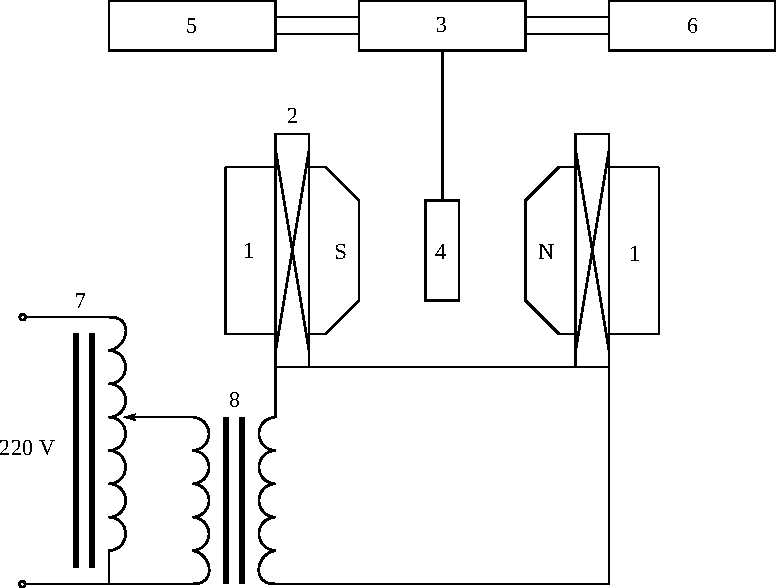
\includegraphics[width=80mm]{drawing.pdf}
\caption{\label{fig:ins}%
实验装置的示意图.$\beta$粒子首先从Sr-Y源中被放射出来,进入在均匀磁场之%
中的真空盒中运动半个圆周之后在真空室下壁上形成一个能谱,能谱各处的对应粒子能量可由圆%
周运动的半径计算.最后再使用闪烁探头在能谱上测量$\beta$粒子的动能,并输%
入多道分析器分析.}
\end{figure}

图~\ref{fig:ins}即是上述实验装置的一个结构示意图.

下面对于实验装置的各部分再进行分别说明.

\subsection{$\beta$粒子源}

$\beta$衰变是放射性核素放射出$\beta$粒子而变为原子序数差1、质量数相同的
核素的过程.$\beta$粒子的本质是高能电子.由于$\beta$衰变中释放出来的中微
子的存在,$\beta$衰变的能谱通常是连续谱.

本实验使用的$\beta$粒子源为$^{90}_{38}\text{Sr} -
^{90}_{39}\text{Y}\beta$源,其能谱在0至2.27Mev的范围内是连续的.\cite{Book}

\subsection{$\beta$磁谱仪}

$\beta$磁谱仪为测量$\beta$粒子能谱内各能对应动量的装置.它利用了带电粒
子在磁场中的运动,将具有不同能量的离子束分束为明确的能谱,并把对于动量的
测量转化为对长度的测量,来完成能量和动量的对应测量.

带电粒子在磁场中作圆周运动服从的运动方程为
\begin{equation}
  \label{eq:Beq}
  \frac{d\bm{p}}{dt} = e\bm{v}\times\bm{B}
\end{equation}
由此方程可解得,粒子动量大小与其做圆周运动的轨道半径的关系
\begin{equation}
  \label{eq:p-R}
  p = eBR
\end{equation}
此即是磁谱仪的原理公式.

\subsection{闪烁探头与多道分析器}

经过磁谱仪中圆周运动的$\beta$粒子,将会打到闪烁探头上,使得闪烁探头送出
一个光信号,该信号会经过光电倍增管转化为电信号并放大,然后进一步被放大电
路放大,成为被多道分析器采集的一个信号.多道分析器在各信号强度上测量信号
计数,便可以得到能谱.

多道分析器接收到的信号强度,即多道分析器采集到的信号道数,与闪烁探头实际
测量到的动能之间的关系,可以认为是线性的.即
\begin{equation}
  \label{eq:E-n}
  E_1 = a + bn
\end{equation}
但是,这一线性关系的系数,是受光电倍增管加的高压电压值和放大电路的放大倍
数影响的,因此,在实际测量中,应当在正式测量前使用标准放射源进行定标,确定
下$a,b$的值.

另一方面,在实验中,在磁场中运动的$\beta$粒子在被闪烁探头接收到之前,会先
后通过真空盒的的一层有机薄膜和闪烁探头的Al窗,他们都会吸收一部分动能,因
此最后探头测得的动能值要经过修正后,才能够认为是可靠的在磁场中运动的电
子的动能.相关的数据修正表见\cite{Book}.

\section{实验结果及分析讨论}

实验的正式测量前,调节完毕后,先使用放射源$^{137}\text{Cs}$和
$^{60}\text{Co}$的几个已知能量峰对闪烁体探测器进行了定标,定标结果如
图~\ref{fig:plot1}所示.

\begin{figure}[htbp]
  \centering
\includegraphics[width=0.8\textwidth]{plot1.pdf}
\caption{\label{fig:plot1}%
此图为闪烁探测器的定标图线,为最小二乘法作$E_k - n$关系线性拟合的结果.拟%
合模型为$E_k = a + bn$,拟合的数值结果为$a = 0.0293648982246, b =%
0.00332429641018, r = 0.999946976185$}
\end{figure}


定标后,首先在真空室中抽真空的情况下进行了实际实验的测量,在磁谱仪的不同
位置使用闪光传感器测放射线的能量峰位置,最终数据如表~\ref{tab:table1}所
示.


\begin{table}[htbp]
  \caption{\label{tab:table1}%
此表为测量数据的具体值与处理值的表格,采用了前述标定的数据,通过峰值道数
计算探测动能,然后通过前述的修正数据得到修正后动能.实验室也记录了磁场强
度为579.7Gs,$\beta$源位置为6.00cm.通过这些数据,计算出了表中的动量值}
\begin{ruledtabular}
  \begin{tabular}{llllll}
     峰值道数 $n$ & 探测动能 $E_k'$/MeV & 修正后动能  $E_k$/MeV & 探头
     位置 $x$/cm & 半径 $R$/cm & 动量 $pc$/MeV\\
     \colrule
     469.0 & 1.588 & 1.680 & 31.00 & 12.50 & 2.174 \\
404 & 1.372 & 1.466 & 28.50 & 11.25 & 1.956 \\
341 & 1.163 & 1.258 & 26.00 & 10.00 & 1.739 \\
277 & 0.950 & 0.994 & 23.50 & 8.75 & 1.522 \\
210 & 0.727 & 0.824 & 21.00 & 7.50 & 1.304 \\
148 & 0.521 & 0.624 & 18.50 & 6.25 & 1.087 \\
83 & 0.305 & 0.424 & 16.00 & 5.00 & 0.870 \\
32 & 0.136 & 0.282 & 13.50 & 3.75 & 0.652 
\end{tabular}
\end{ruledtabular}
\end{table}


测量数据与狭义相对论理论预计、经典力学的理论预计曲线的对比图参见
图~\ref{fig:plot2}

\begin{figure}[htbp]
  \centering
\includegraphics[width=0.8\textwidth]{plot2.pdf}
\caption{\label{fig:plot2}%
此图为实验测得值与理论曲线的比较图,图中蓝线为狭义相对论理论曲线,曲线公
式为$pc/\text{MeV} = [(E_k/\text{MeV} + 0.511)^2 - 0.511^2]^{1/2}$.红
线为经典力学理论曲线,曲线公式为$pc/\text{MeV} = (1.022E_k/\text{MeV})^{1/2}$}
\end{figure}

图~\ref{fig:plot2}中的测量数据表明,实验的结果很好的吻合了狭义相对论理
论对于高速运动物体的动量-动能关系的预计,并且也同样说明了经典力学的理论
在这样的高速运动物体上的不适用性.


第一组实验的测量结束后,在真空室中不是真空状态,即在有空气的条件下,其他
所有的实验条件和实验室参数都不变,进行了第二组实验数据的测量与处理,数据
请参见表~\ref{tab:table2}.


\begin{table}[htbp]
  \caption{\label{tab:table2}%
此表为测量数据的具体值与处理值的表格,数据处理方式与和其他实验室参数与前
述完全相同,但此组数据是在真空室中不为真空,即有空气的条件下完成实验和测
量的}
\begin{ruledtabular}
  \begin{tabular}{llllll}
     峰值道数 $n$ & 探测动能 $E_k'$/MeV & 修正后动能  $E_k$/MeV & 探头
     位置 $x$/cm & 半径 $R$/cm & 动量 $pc$/MeV\\
     \colrule
94 & 0.342 & 0.458 & 16.00 & 5.00 & 0.870 \\
150 & 0.528 & 0.629 & 18.50 & 6.25 & 1.087 \\
208 & 0.721 & 0.818 & 21.00 & 7.50 & 1.304 \\
274 & 0.940 & 1.036 & 23.50 & 8.75 & 1.522 \\
318 & 1.086 & 1.178 & 26.00 & 10.00 & 1.739
   \end{tabular}
\end{ruledtabular}
\end{table}

同样,在这组数据上,可以作出实验测得值与两种理论预言结果的对比图,如
图~\ref{fig:plot3}所示.同样,这幅图也可以说明在高速运动的物体上,相对论
理论的适用性与经典力学理论的不适用性.但是,在这幅图中,在动能较高的粒子
段上,实验测得的动量结果对于理论有着系统的偏大现象.这一现象应该可以解释
为:由于空气的存在,$\beta$粒子在运动中撞击空气分子而损失能量.这一现象导致了对于
某一能量的分子,由于其前段运动在高能量高动量的较大运动半径下完成,从而使得测
得的半径值,即粒子出射时运动半径值与到达探测器时运动半径值的算数平均值,
比粒子最后抵达探测器时的运动半径值要偏大的情况.而这一情况也就导致了动
量测量值的偏大.

另一方面,能量越高粒子动量偏差值越大,正说明了能量越高的粒子在空气中损失的
能量也越多.

\begin{figure}[htbp]
  \centering
\includegraphics[width=0.8\textwidth]{plot3.pdf}
\caption{\label{fig:plot3}%
此图为实验测得值与理论曲线的比较图,数据处理方式和其他实验室参数与前
述完全相同,但此组数据是在真空室中不为真空,即有空气的条件下完成实验和测
量的.图中蓝线为狭义相对论理论曲线,红线为经典力学理论曲线.}
\end{figure}


\section{结论}

实验通过对于高能$\beta$粒子动量和动能的关系测量,验证了狭义相对论理论中
粒子动量-动能关系的有效性,从而验证了狭义相对论理论对于高速运动物体的适
用性.另一方面,实验也验证了经典力学动量-动能关系的不适用性,从而验证了经
典力学理论对于高速运动物体的不适用性.

另一方面,实验通过对于$\beta$粒子在空气运动后的动量-动能关系测量,验证了
$\beta$粒子在空气中运动时会损失能量,而且粒子的能量越高能量的损失值越高
的这一事实.

\section{致谢}

感谢王思广老师在实验中认真而专业的指导.

感谢孙思白学长提供的实验报告模板和报告格式作为参考.

% Bibliography example.
\begin{thebibliography}{}
\bibitem{Book} 吴思成,王祖铨~2010 近代物理实验(第三版)(北京:高等教
育出版社)第107页.  %实验书
\bibitem{report} 孙思白~北京大学2014年近代物理实验报告:扫描隧穿显微镜
  观察高定向热解石墨的原子尺度图像
 %同学实验报告
\end{thebibliography}

\clearpage
\appendix
\section{思考题}

\begin{enumerate}
\item 实验中射入均匀磁场中的$\beta$粒子速度方向实际上有一定的角分布,请
  考虑这一因素对实验结果的影响

  这一角分布将导致对于磁谱仪的能谱上面的每一点,接收到的粒子将不会是单
  一能量的,而会有一个连续的能量分布.这将会对峰位置的判定引入误差,从而
  对实验结果引入一定误差

\item 磁体边缘的磁场强度较中心区域弱,请半定量分析其对$\beta$粒子动量测
  量的影响

  根据公式~\ref{eq:p-R},这将会导致测得的半径值较实际半径值大,从而导致
  测得的动量值较实际值偏大.
\end{enumerate}

\end{document}